\documentclass{article}

\usepackage[margin=1in]{geometry}

\usepackage{lmodern}
\usepackage{amsmath}
\usepackage{amssymb}
\usepackage{upgreek}
\usepackage{pgfplots}
\usepackage{qtree}
\usepackage{calc}
\usepackage[normalem]{ulem}
\usepackage[utf8]{inputenc}
\usepackage[T1]{fontenc}

\pgfplotsset{compat=1.11}
\usetikzlibrary{arrows, decorations.markings}
\usetikzlibrary{3d}
\usetikzlibrary{shapes.geometric,decorations.fractals,shadows}
\usepgfplotslibrary{polar}


\begin{document}

\section{Curvas Parametrizadas}
De modo geral, podemos descrever uma curva plana por uma \uline{parametrização}:
\[ \vec{r}(t) = (x(t), y(t)) \qquad \text{onde $x(t)$ e $y(t)$ são funções da variável $t$.} \]
Exemplo: \\[-5pt]

$y = 2x \quad \rightarrow \quad \vec{r}(t) = (t, 2t)$

\subsection{Vetor Tangente}
O vetor \uline{tangente} \`a curva $\vec{r}(t) = (x(t),\, y(t))$ em um ponto $(x(t_\uplambda),\, y(t_\uplambda))$ é:
\[ \vec{v}(t_\uplambda) = \vec{x}\,'(t_\uplambda)\vec{\dot{\imath}} \> + \> \vec{y}\,'(t_\uplambda)\vec{\dot{\jmath}} \]
Denota-se $\vec{r}\,'(t_\uplambda)$. \\[5pt]
Exemplo:

Vetor tangente \`a curva $\vec{r}(t) = (t,\, 2t)$ no ponto $(3, 6)$:
\begin{gather*}
  (3, 6) \>\Rightarrow\> t_\uplambda = 3 \\[5pt]
  \vec{x}\,'(t) = 1 \\
  \vec{y}\,'(t) = 2 \\
  \therefore \\
  \vec{v}\,'(3) = \vec{\dot{\imath}} + 2\vec{\dot{\jmath}}
\end{gather*}
O respectivo vale para curvas no espaço.

\subsection{Gráficos}

\begin{tabular}{cc}
  $\vec{r}(t) = (\cos t, 0, \sin t)$ & $\vec{r}(t) = (\cos t, \sin t, t)$ \\[5pt]
  \vtop{\null\hbox{
    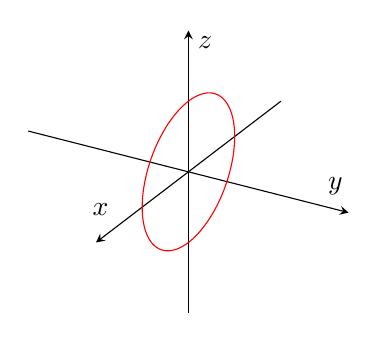
\begin{tikzpicture}
      \begin{axis}[
          view       = {120}{30},
          axis lines = middle,
          xlabel     = $x$,
          ylabel     = $y$,
          zlabel     = $z$,
          zmax       = 2,
          zmin       = -2,
          xmax       = 2,
          xmin       = -2,
          height     = 8cm,
          width      = 8cm,
          xtick      = \empty,
          ytick      = \empty,
          ztick      = \empty
        ]
        \addplot3+ [
          domain    = 0:2*pi,
          samples   = 100,
          samples y = 0,
          mark      = none,
          red,
        ]
        ( {cos(deg(x))}, {0}, {sin(deg(x))} );
      \end{axis}
    \end{tikzpicture}
  }}
  &
  \qquad\vtop{\null\hbox{
    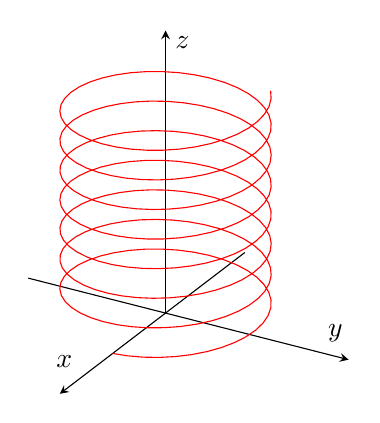
\begin{tikzpicture}
      \begin{axis}[
          view       = {120}{30},
          axis lines = middle,
          xlabel     = $x$,
          ylabel     = $y$,
          zlabel     = $z$,
          zmax       = 60,
          xmax       = 2,
          xmin       = -1.5,
          ymax       = 2,
          ymin       = -1.5,
          height     = 8cm,
          width      = 8cm,
          xtick      = \empty,
          ytick      = \empty,
          ztick      = \empty
        ]
        \addplot3+ [
          domain     = 0:14.7*pi,
          samples    = 300,
          samples y  = 0,
          mark       = none,
          red,
        ]
        ( {cos(deg(x))},{sin(deg(x))},{x});
      \end{axis}
    \end{tikzpicture}
  }}
\end{tabular}


\pagebreak
\subsection{Comprimento de Curvas}
O comprimento de uma curva $\boldsymbol{\gamma}(t)$ no plano é dado por
\begin{align*}
  l(\boldsymbol{\gamma}(t)) \quad &= \quad
  \lim_{\Delta t \to 0} { \sum_i \sqrt{ {\left(\frac{x(t_{i+1}) - x(t_i)}{\Delta t}\right)}^2 + { \left(\frac {y(t_{i+1}) - y(t_i)}{\Delta t}\right) }^2 } \cdot \Delta t } \\
  &= \quad \int\limits_a^b \sqrt{{(x'(t))}^2 + {(y'(t))}^2} \cdot dt
\end{align*}
Para uma curva $\boldsymbol{\gamma}(t)$ no espaço, analogamente:
\[ l(\boldsymbol{\gamma}(t)) = \int\limits_a^b \sqrt{{(x'(t))}^2 + {(y'(t))}^2 + {(z'(t))}^2} \cdot dt \]
Exemplo:
\begin{figure}[!h]
  \qquad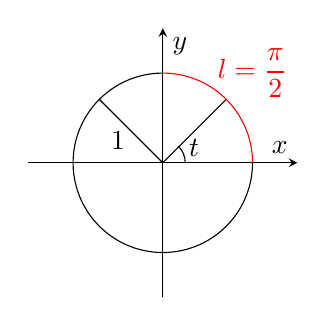
\begin{tikzpicture}
    \begin{axis}[
        axis lines = center,
        xmax       = 1.5,
        xmin       = -1.5,
        ymax       = 1.5,
        ymin       = -1.5,
        height     = 5cm,
        width      = 5cm,
        xtick      = \empty,
        ytick      = \empty,
        xlabel     = $x$,
        ylabel     = $y$,
        black
      ]
      \addplot [
        domain=pi/2:2*pi,
        samples=150,
        black
      ] ({cos(deg(x))}, {sin(deg(x))});
      \addplot [
        domain = -sqrt(2)/2 : sqrt(2)/2,
        samples = 100,
        black
      ] {abs(x)};
      \addplot [
        domain=0:pi/2,
        samples= 50,
        red
      ] ({cos(deg(x))}, {sin(deg(x))});
      
      \node at (-0.5, 0.25) {$1$};
      
      \draw (axis cs:.25,0) arc [radius=.3cm,start angle=0,end angle=45];
      \node at (0.35, 0.17) {$t$};
      
      \node [red] at (1, 1) {$l = \dfrac{\pi}{2}$};
    \end{axis}
  \end{tikzpicture}
\end{figure}

$\boldsymbol{\gamma}(t) = (\cos t, \sin t)$ \\[-5pt]

Obtemos o arco acima variando $t$ entre $a = 0$ e $b = \dfrac{\pi}{2}$. \\[-5pt]

Logo
\begin{align*}
  l &= \int\limits_0^{\pi/2} \sqrt{ {(-\sin t)}^2 + {(\cos t)}^2 } \cdot dt \\
  &= \int\limits_0^{\pi/2} 1 \cdot dt \\[1pt]
  &= \frac{\pi}{2}
\end{align*}



\pagebreak
\section{Coordenadas Polares}
Um ponto em coordenadas polares é definido por um raio e um ângulo:
\[ p = {(r, \theta)}_{polar} \]

\begin{tabbing}
  Exemplo: \= Se $p = {\left(5, \frac{\pi}{4}\right)}_{polar}$ \\
  \>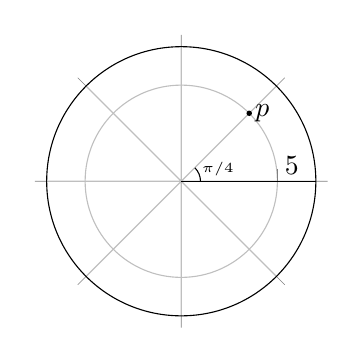
\begin{tikzpicture}
    \begin{polaraxis} [
        ymax = 7,
        height = 5cm,
        width  = 5cm,
        ytick={5},
        xticklabel = \empty,
        yticklabel = \empty,
      ]
      \node [circle,fill,inner sep=.7pt] at (45, 5) {};
      \node at (40, 5.5) {$p$};
      \draw (axis cs:0,1) arc [radius=.24cm,start angle=0,end angle=45];
      
      \node at (18, 2) {\tiny $\pi/4$};
      \node at (8, 5.8) {$5$};
    \end{polaraxis}
  \end{tikzpicture}
\end{tabbing}
\underline{Convenções}:
\begin{itemize}
  \item $\theta > 0$ se medido, a partir do eixo polar, no sentido anti-horário.
  \item $\theta < 0$ se medido, a partir do eixo polar, no sentido horário.
  \item ${(-r, \theta)}_{polar} = {(r, \theta + \pi)}_{polar}$ \\ [5pt]
    Exemplo: $(-3, \dfrac{\pi}{4}) = (3, \dfrac{5\pi}{4})$ \\
    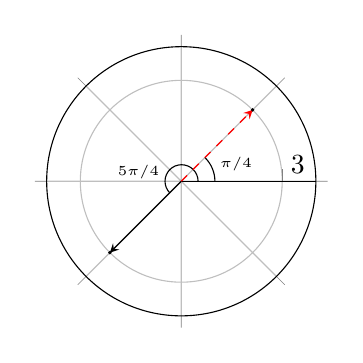
\begin{tikzpicture}
    \begin{polaraxis} [
        ymax = 4,
        height = 5cm,
        width  = 5cm,
        ytick={3},
        xticklabel = \empty,
        yticklabel = \empty,
      ]
      \draw [>=stealth,->] (0,0) -- (225, 3);
      \node [circle,fill,inner sep=.5pt] at (225, 3) {};
      \draw (axis cs:0, 0.5) arc [radius=.21cm,start angle=0,end angle=225];
      \node at (168, 1.3) {\tiny $5\pi/4$};

      \draw [>=stealth,->, red, dashed] (0,0) -- (45, 3);
      \node [circle,fill,inner sep=.5pt] at (45, 3) {};
      \draw (axis cs:0,1) arc [radius=.42cm,start angle=0,end angle=45];
      \node at (17, 1.7) {\tiny $\pi/4$};
      
      \node at (8, 3.5) {$3$};
    \end{polaraxis}
  \end{tikzpicture}
  \item $\forall \theta: {(0, \theta)}_{polar} = 0$
\end{itemize}

\subsection{Relação Entre Sistemas de Coordenadas}
\begin{figure}[!h]
  \centering
  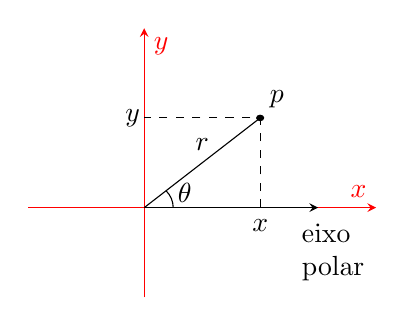
\begin{tikzpicture}
    \begin{axis}[
        axis lines = center,
        xlabel     = $x$,
        ylabel     = $y$,
        xmax       = 2,
        xmin       = -1,
        ymax       = 2,
        ymin       = -1,
        height     = 5cm,
        width      = 6cm,
        xtick      = \empty,
        ytick      = \empty,
        red
      ]
      \addplot [
        domain=0:1,
        samples=200,
        black
      ] {x};
      
      \node [black] at (0.5, 0.7) {$r$};
      
      \draw [black, dashed] (axis cs: 1, 0) |- (axis cs: 0, 1);
      \node [black] at (1, -0.2) {$x$};
      \node [black] at (-0.1, 1) {$y$};
  
      \draw [black] (axis cs:.25,0) arc [radius=.3cm,start angle=0,end angle=45];
      \node [black] at (0.35, 0.17) {$\small\theta$};
      
      \draw [>=stealth,->, black] (0,0) -- (1.5,0);
      \node [black, text width=1cm] at (1.7, -0.5) {eixo polar};
  
      \draw [black, fill=black] (1,1) circle (0.03) node[above right] {$p$};
    \end{axis}
  \end{tikzpicture}
\end{figure}
\vspace{-15pt}
\[ p = {(r,\theta)}_{polar} = {(x, y)}_{ret} \]
\begin{alignat*}{3}
  &\forall r, \theta &&: {(r, \theta)}_{polar} &&= {(r \cdot \cos \theta,\, r \cdot \sin \theta)}_{ret} \\
  &\forall x, y &&: {(x, y)}_{ret} &&= {\left(\sqrt{x^2 + y^2},\, \arctan{\frac{y}{x}}\right)}_{polar}
\end{alignat*}

\subsection{Curvas Polares}
Uma curva polar é definida por uma equação entre as coordenadas polares dos pontos da curva (equação polar). \\

\begin{tabbing}
  Exemplos: \= $r^2 + e^{r\theta} = 0$ \\[5pt]
  \> $0 \cdot \theta + r - 25 = 0 \quad\Rightarrow\quad r = 25$ \\
  \>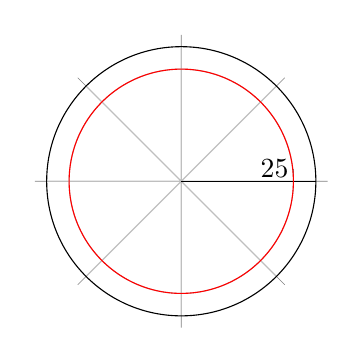
\begin{tikzpicture}
    \begin{polaraxis} [
        ymax = 30,
        height = 5cm,
        width  = 5cm,
        ytick={25},
        xticklabel = \empty,
        yticklabel = \empty,
      ]
      \addplot [
        domain=0:360,
        samples=200,
        red
      ] {25};
      
      \node at (8, 21) {$25$};
    \end{polaraxis}
  \end{tikzpicture} \\[5pt]
  \> $\theta + \frac{\pi}{6} = 0 \quad\Rightarrow\quad \theta = -\frac{\pi}{6}$ \\
  \>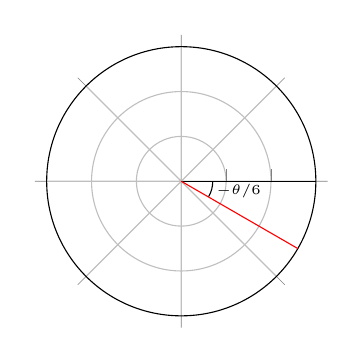
\begin{tikzpicture}
    \begin{polaraxis} [
        ymax = 3,
        height = 5cm,
        width  = 5cm,
        ytick  = {1,2},
        xticklabel = \empty,
        yticklabel = \empty,
      ]
      \addplot [
        domain=0:360,
        samples=200,
        red
      ] ({deg(-pi/6)}, {x});
      
      \draw [black] (axis cs: 331, .7) arc [radius=.38cm,start angle=330,end angle=360];
      \node at (350, 1.3) {\tiny $-\theta/6$};
    \end{polaraxis}
  \end{tikzpicture} \\[5pt]
  \> $r = \cos{(2\theta)}$ \\[5pt]
  \>\quad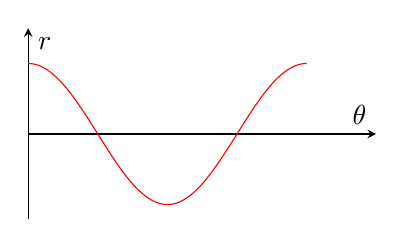
\begin{tikzpicture}
      \begin{axis}[
          axis lines = middle,
          xlabel     = $\theta$,
          ylabel     = $r$,
          xmax       = 3*pi,
          xmin       = pi/2,
          ymax       = 1.5,
          ymin       = -1.2,
          height     = 4cm,
          width      = 6cm,
          xtick      = \empty,
          ytick      = \empty,
        ]
        \addplot [
          domain=0:5*pi/2,
          samples=200,
          red
        ] {sin(deg(x))};
      \end{axis}
  \end{tikzpicture} \\
  \>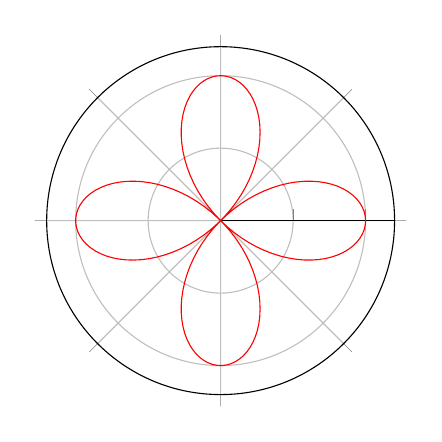
\begin{tikzpicture}
    \begin{polaraxis} [
        ymax = 1.2,
        height = 6cm,
        width  = 6cm,
        ytick  = {0.5,1},
        xticklabel = \empty,
        yticklabel = \empty,
      ]
      \addplot [
        domain=0:360,
        samples=200,
        red
      ] {cos(2*x)};
    \end{polaraxis}
  \end{tikzpicture}
\end{tabbing}



\pagebreak
\section{Superfícies}
Qual é o conjunto solução da equação $x^2 + y^2 + z^2 = 4$? \\[5pt]
Resposta: uma esfera de raio 2 centrada na origem. \\[5pt]
\begin{figure}[h]
  \centering
  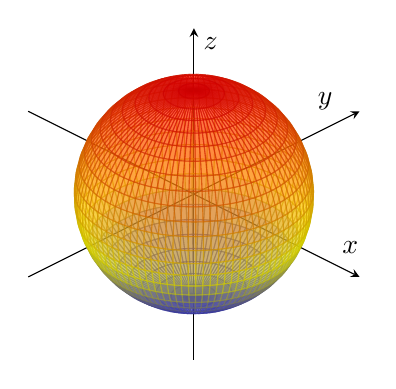
\begin{tikzpicture}
    \begin{axis}[%
        view/h = 45,
        axis equal,
        width=10cm,
        height=10cm,
        axis lines = center,
        xlabel = {$x$},
        ylabel = {$y$},
        zlabel = {$z$},
        ticks=none,
        enlargelimits=0.3,
      ]
      \addplot3[%
        opacity = 0.5,
        surf,
        z buffer = sort,
        samples = 50,
        variable = \u,
        variable y = \v,
        domain = 0:180,
        y domain = 0:360,
      ]
      ({cos(u)*sin(v)}, {sin(u)*sin(v)}, {cos(v)});
    \end{axis}
  \end{tikzpicture}
\end{figure}


\subsection{Estratégias de esboço de superfícies no espaço}
Identificar sua interseção com planos (cortes) que cobrem todo o espaço. \\[-10pt]
\begin{tabbing}
  Exemplo: \= $S = \left\{ (x, y, z) \in \mathbb{R}^3 \enspace \bigg| \enspace \dfrac{x^2}{25} + \dfrac{y^2}{4} + \dfrac{z^2}{9} = 1 \right\}$ \\[5pt]
  \> Cortes horizontais: \\[-5pt]
  \>\begin{minipage}{.5 \textwidth}
    \begin{align*}
      C_h &= S \cap \Pi_h\{ \text{Plano horizontal de altura $h$} \} \\
      &= S \cap \Pi_h\left\{ (x, y, z) \in \mathbb{R}^3 \enspace \big| \enspace z = h \right\} \\
      &= \left\{ (x, y, z) \in \mathbb{R}^3 \enspace \bigg| \enspace \dfrac{x^2}{25} + \dfrac{y^2}{4} + \dfrac{h^2}{9} = 1 \right\}
    \end{align*}
  \end{minipage}\\
  \> Para\\[-10pt]
  \>\quad\begin{minipage}{.35 \textwidth}
    \begin{alignat*}{2}
      &h > 3   \enspace &&: \enspace S \cap \Pi_h = \varnothing \\[5pt]
      &h = 3   \enspace &&: \enspace S \cap \Pi_3 = \left\{ (0,0,3) \right\} \\[5pt]
      &h < -3  \enspace &&: \enspace S \cap \Pi_h = \varnothing \\[5pt]
      &h = -3  \enspace &&: \enspace S \cap \Pi_{-3} = \left\{ (0,0,-3) \right\} \\[5pt]
      &|h| < 3 \enspace &&: \enspace S \cap \Pi_h \\[-5pt]
      & &&: \enspace \text{Plano xz} \rightarrow S \cap \left\{ y = 0 \right\} \Rightarrow \left\{ (x, 0, z) \in \mathbb{R}^3 \enspace \bigg| \enspace \dfrac{x^2}{25} + \dfrac{z^2}{9} = 1 \right\} \therefore \text{Elipse} \\
      & &&: \enspace \text{Plano yz} \rightarrow S \cap \left\{ x = 0 \right\} \Rightarrow \left\{ (0, y, z) \in \mathbb{R}^3 \enspace \bigg| \enspace \dfrac{y^2}{4} + \dfrac{z^2}{9} = 1 \right\} \therefore \text{Elipse}
    \end{alignat*}
  \end{minipage}\\[10pt]
  \> Portanto, a superfície é um elipsóide de altura 6 e diâmetros 10 e 4.
\end{tabbing}


\pagebreak

\subsection{Cilindros}
Um cilindro é um objeto construido através de uma curva $\boldsymbol{\gamma}$ no plano e um ângulo $\alpha$. \\[5pt]
O cilindro é o conjunto de todas as retas que possuem interseção com $\boldsymbol{\gamma}$, formando um ângulo equivalente \`a $\alpha$ com o plano de $\boldsymbol{\gamma}$. \\[10pt]
Qual é a superfície descrita pela equação $x^2 + y^2 = 9$? \\[5pt]
Qual é o objeto geométrico $\{ (x, y, z) \in \mathbb{R}^3 \> | \> x^2 + y^2 = 9 \}$? \\[5pt]
Resposta: \uline{Cilindro}. O conjunto é formado por todos os pontos do espaço cuja distância ao eixo $z$ é $3$. \\[-5pt]
\begin{figure}[!h]
  \centering
  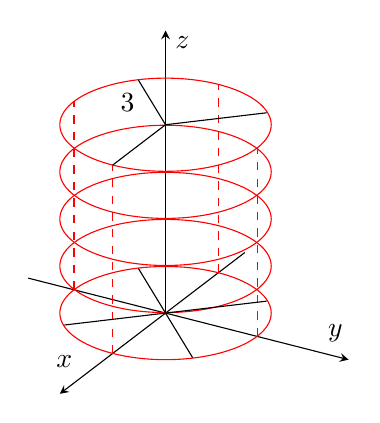
\begin{tikzpicture}
    \begin{axis}[
        view       = {120}{30},
        axis lines = middle,
        xlabel     = $x$,
        ylabel     = $y$,
        zlabel     = $z$,
        zmax       = 60,
        xmax       = 2,
        xmin       = -1.5,
        ymax       = 2,
        ymin       = -1.5,
        height     = 8cm,
        width      = 8cm,
        xtick      = \empty,
        ytick      = \empty,
        ztick      = \empty
      ]
      \addplot3+ [
        domain    = 0:2*pi,
        samples   = 100,
        samples y = 0,
        mark      = none,
        red,
      ]
      ( {cos(deg(x))}, {sin(deg(x))}, {0} );
      \addplot3+ [
        domain    = 0:2*pi,
        samples   = 100,
        samples y = 0,
        mark      = none,
        red,
      ]
      ( {cos(deg(x))}, {sin(deg(x))}, {10} );
      \addplot3+ [
        domain    = 0:2*pi,
        samples   = 100,
        samples y = 0,
        mark      = none,
        red,
      ]
      ( {cos(deg(x))}, {sin(deg(x))}, {20} );
      \addplot3+ [
        domain    = 0:2*pi,
        samples   = 100,
        samples y = 0,
        mark      = none,
        red,
      ]
      ( {cos(deg(x))}, {sin(deg(x))}, {30} );
      \addplot3+ [
        domain    = 0:2*pi,
        samples   = 100,
        samples y = 0,
        mark      = none,
        red,
      ]
      ( {cos(deg(x))}, {sin(deg(x))}, {40} );

      \draw [red, dashed] (axis cs: 1, 0, 0)  |- (axis cs: 1, 0, 40);
      \draw [red, dashed] (axis cs: -1, 0, 0) |- (axis cs: -1, 0, 40);
      \draw [red, dashed] (axis cs: 0, 1, 0)  |- (axis cs: 0, 1, 40);
      \draw [red, dashed] (axis cs: 0, -1, 0) |- (axis cs: 0, -1, 40);

      \draw (axis cs: 0, 0, 40) -- (axis cs: 1, 0, 40);
      \draw (axis cs: 0, 0, 40) -- (axis cs: -0.7, 0.7, 40);
      \draw (axis cs: 0, 0, 40) -- (axis cs: -0.7, -0.7, 40);
      \draw (axis cs: 0, 0, 0) -- (axis cs: -0.7, 0.7, 0);
      \draw (axis cs: 0, 0, 0) -- (axis cs: -0.7, -0.7, 0);
      \draw (axis cs: 0, 0, 0) -- (axis cs: 0.7, -0.7, 0);
      \draw (axis cs: 0, 0, 0) -- (axis cs: 0.7, 0.7, 0);
      
      \node at (0.2, -0.3, 45) {3};
    \end{axis}
  \end{tikzpicture}
\end{figure}

\subsection{Quádricas}
As superfícies quádricas são soluções de equações da forma
\[ ax^2 + by^2 + cz^2 \> + \> dxy + eyz + fxz \> + \> gx + hy + iz \> + \> j = 0 \]


\section{Funções de duas ou mais variáveis}
Uma função de 2 variáveis é uma função do tipo
\[ f: D \rightarrow \mathbb{R} \qquad \text{onde} \> D \subseteq \mathbb{R}^2 \]

\subsection{Gráficos}
O gráfico de uma função $f: D \rightarrow \mathbb{R}$ de duas variáveis é o subconjunto de $\mathbb{R}^3$ formado pelos pontos
\[ (x,\, y,\, f(x, y)) \in \mathbb{R}^3 \qquad \text{onde} \> (x,\, y) \in D \]


\subsection{Curvas e Superfícies de Nível}
Uma curva de nível de altura $h$ de uma função $f: D \to \mathbb{R}$ é o conjunto de pontos $(x, y)$ do plano tais que
\[ f(x,y) = h \]


\pagebreak

\subsection{Limite e Continuidade}

\subsubsection{Limite}
Seja uma função $f: D \rightarrow \mathbb{R}$, então define-se
\[ \lim_{(x,y) \to (a,b)} f(x,y) = L \]
Dizemos que $f$ tende a $L$ quando $(x,y)$ tende a $(a,b)$, se $\forall \epsilon > 0$ arbitrário
\begin{alignat*}{2}
  &\exists \delta \> : && \> 0 < \delta < \sqrt{ {(x-a)}^2 + {(y-b)}^2 }\\
                     & && \> \left| f(x,y) - L \right| < \epsilon
\end{alignat*}
As seguintes propriedades valem:
\begin{itemize}
  \item $\lim\limits_{(x,y)\to(a,b)} (f(x,y) + g(x,y)) = \lim\limits_{(x,y)\to(a,b)} f(x,y) + \lim\limits_{(x,y)\to(a,b)} g(x,y) $\\
  \item $\lim\limits_{(x,y)\to(a,b)} (f(x,y) - g(x,y)) = \lim\limits_{(x,y)\to(a,b)} f(x,y) - \lim\limits_{(x,y)\to(a,b)} g(x,y) $\\
  \item $\lim\limits_{(x,y)\to(a,b)} (f(x,y) \cdot g(x,y)) = \lim\limits_{(x,y)\to(a,b)} f(x,y) \> \cdot \lim\limits_{(x,y)\to(a,b)} g(x,y) $\\
  \item $\lim\limits_{(x,y)\to(a,b)} \left( \dfrac{f(x,y)}{g(x,y)} \right) = \dfrac{\lim\limits_{(x,y)\to(a,b)} f(x,y)}{\lim\limits_{(x,y)\to(a,b)} g(x,y)} $\\
\end{itemize}
\vspace{30pt}
Seja $\gamma(t) = (x(t), y(t))$ qualquer curva parametrizada com
\[ \lim_{t\to0} \gamma(t) = (\lim_{t\to0} x(t), \lim_{t\to0} y(t)) = (a,b) \]
Se $\lim\limits_{(x,y)\to(a,b)} f(x,y) = L$, então para toda curva $\gamma$ vale:\\[-5pt]
\[ \lim_{t\to0} f(x(t), y(t)) = L \]
\vspace{30pt}\\
Seja uma função $f$ e duas curvas $\gamma$ e $\widetilde\gamma$ quaisquer no domínio de $f$ tais que
\[ \lim_{t \to 0} \gamma(t) = \lim_{t \to 0} \widetilde\gamma(t) = (a,b) \]
Se $\lim\limits_{(x,y) \to (a,b)} f(x,y)$ existe, então pra toda $\gamma$ e $\widetilde\gamma$:\\[-5pt]
\[ \lim_{t \to 0} f(x(t), y(t)) \> = \> \lim_{t \to 0} f(\widetilde{x}(t), \widetilde{y}(t)) \]

\pagebreak

\begin{tabbing}
  Exemplos:\enspace\= $f(x,y) = 5 \quad \Rightarrow \quad \lim\limits_{(x,y) \to (3,-1)} f(x,y) = 5$ \\[10pt]
  \> $f(x,y) = x \quad \Rightarrow \quad \lim\limits_{(x,y) \to (8,-6)} f(x,y) = 8$ \\[10pt]
  \> $f(x,y) = \dfrac{x^2 - y^2}{x^2 + y^2} \enspace \left(D: \mathbb{R}^2 - \{ (0,0) \} \right) \quad \Rightarrow \quad \nexists \lim\limits_{(x,y) \to (0,0)} f(x,y) $ pois: \\[5pt]
  \>\quad\begin{minipage}{400px}
      Seja $\gamma(t) = (t, 0)$ a reta sobre o eixo $x$, e $\widetilde{\gamma}(t) = (0, t)$ a reta sobre o eixo $y$.
      \begin{alignat*}{4}
        \lim_{t\to0} f(x(t), y(t)) &= \lim_{t\to0} f(t, 0) &&= \lim_{t\to0} \frac{t^2 - 0^2}{t^2 + 0^2} &&= 1\\[5pt]
        \lim_{t\to0} f(\widetilde{x}(t), \widetilde{y}(t)) &= \lim_{t\to0} f(0, t) &&= \lim_{t\to0} \frac{0^2 - t^2}{0^2 + t^2} &&= -1
      \end{alignat*}
      \[ 1 \neq -1 \]
      \centering
      \begin{tikzpicture}
        \begin{axis}[
            axis lines = center,
            xmax       = 1.5,
            xmin       = -1.5,
            ymax       = 1.5,
            ymin       = -1.5,
            height     = 4cm,
            width      = 4cm,
            xtick      = \empty,
            ytick      = \empty,
            xlabel     = $x$,
            ylabel     = $y$,
            black
          ]
          \draw [red, ->, >=stealth] (1,0) -- (0.2, 0);
          \draw [red, ->, >=stealth] (-1,0) -- (-0.2, 0);
          
          \draw [teal, ->, >=stealth] (0,1) -- (0, 0.2);
          \draw [teal, ->, >=stealth] (0,-1) -- (0, -0.2);
          
          \node [red] at (0.6, -0.3) {$\gamma$};
          \node [teal] at (0.3, 0.6) {$\widetilde{\gamma}$};
        \end{axis}
      \end{tikzpicture}
    \end{minipage} \\[10pt]
  \> $f(x,y) = \dfrac{xy^2}{x^2 + y^4} \enspace \left(D: \mathbb{R}^2 - \{ (0,0) \} \right) \quad \Rightarrow \quad \nexists \lim\limits_{(x,y) \to (0,0)} f(x,y) $ pois: \\[5pt]
  \>\quad\begin{minipage}{400px}
      Seja $\gamma(t) = (t, \alpha t)$, e $\widetilde{\gamma}(t) = (t^2, t)$.
      \begin{alignat*}{4}
        \lim_{t\to0} f(x(t), y(t)) &= \lim_{t\to0} f(t, \alpha t) &&= \lim_{t\to0} \frac{t \cdot{(\alpha t)}^2}{t^2 + {(\alpha t)}^4} &&= 0\\[5pt]
        \lim_{t\to0} f(\widetilde{x}(t), \widetilde{y}(t)) &= \lim_{t\to0} f(t^2, t) &&= \lim_{t\to0} \frac{t^2 \cdot {(t)}^2}{{(t^2)}^2 + t^4} &&= \frac{1}{2}
      \end{alignat*}
      \[ 0 \neq \frac{1}{2} \]
      \centering
      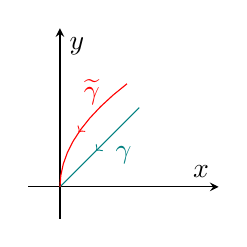
\begin{tikzpicture}
        \begin{axis}[
            axis lines = center,
            xmax       = 1,
            xmin       = -0.2,
            ymax       = 1,
            ymin       = -0.2,
            height     = 4cm,
            width      = 4cm,
            xtick      = \empty,
            ytick      = \empty,
            xlabel     = $x$,
            ylabel     = $y$,
            black
          ]
          \addplot [
            domain = 0 : 0.5,
            samples = 10,
            postaction={
              decorate,
              decoration={
                markings,
                mark = at position 0.5 with {\arrow{<}}
              }
            },
            teal
          ] {x};
          \addplot [
            domain = 0 : 0.65,
            samples = 10,
            postaction={
              decorate,
              decoration={
                markings,
                mark = at position 0.5 with {\arrow{<}}
              }
            },
            red
          ] ({x^2}, {x});
          \node [teal] at (0.4, 0.2) {$\gamma$};
          \node [red] at (0.2, 0.6) {$\widetilde{\gamma}$};
        \end{axis}
      \end{tikzpicture}
    \end{minipage} \\[10pt]
\end{tabbing}

\subsubsection{Continuidade}
Dizemos que $f$ é contínua em $(a,b)$ se
\[ \lim_{(x,y) \to (a,b)} f(x,y) = f(a,b) \]
Dizemos que $f$ é contínua se é contínua em todos os pontos de seu domínio.
\begin{tabbing}
  Propriedades: \= A composição de duas funções contínuas é contínua.\\
  \> $f(x,y) = c$ é contínua.\\
  \> $f(x,y) = x$ é contínua.\\
  \> $f(x,y) = y$ é contínua.
\end{tabbing}


\pagebreak


\subsection{Derivadas Parciais}
A derivada parcial de uma função de $n$ variáveis $f(\lambda_1, \hdots, \lambda_n)$ com relação a uma variável $\lambda_\alpha$, no ponto $(a_1, \> \hdots \> , a_n)$ é:
\[ \lim_{\Delta \lambda_\alpha \to 0} \frac{f(a_1, \> \hdots \> , a_\alpha + \Delta \lambda_\alpha, \> \hdots \> , a_n) - f(a_1, \> \hdots \> , a_n)}{\Delta \lambda_\alpha} \]
Para uma função de 2 variáveis $f(x,y)$ no ponto $(a, b)$, por exemplo:
\begin{align*}
  \text{Em relação a}\ x:& \quad \lim_{\Delta x \to 0} \frac{f(a + \Delta x, b) - f(a, b)}{\Delta x} \\[5pt]
  \text{Em relação a}\ y:& \quad \lim_{\Delta y \to 0} \frac{f(a + \Delta y, b) - f(a, b)}{\Delta y}
\end{align*}
Há três nomenclaturas convencionais, para a variável x por exemplo:
\begin{itemize}
\item{\makebox[2cm][l]{$\dfrac{\delta f}{\delta x} (a,b)$} Fração indicando a variável sobre qual foi a derivada parcial.}
\item{\makebox[2cm][l]{$f_x(a, b)$} Em ordem $\leftarrow$, subscrito em $f$ a variável sobre qual foi a derivada parcial.}
\item{\makebox[2cm][l]{$D_1f(a,b)$} Em ordem $\rightarrow$, subscrito em $D$ o índice da variável sobre qual foi a derivada parcial.}
\end{itemize}

\subsubsection{Cálculo operacional da dervivada parcial}
Para derivar parcialmente com relação a uma variável, basta considerar as demais como constantes e derivar normalmente.\\[5pt]
Exemplo: $f(x,y) = x^2y + e^{xy}$
\begin{align*}
  & \Rightarrow f_x(x,y) = (2x)y + e^{xy} \cdot y = 2xy + ye^{xy}&& \\[5pt]
  & \Rightarrow f_y(x,y) = x^2 \cdot 1 + e^{xy}\cdot x = x^2 + xe^{xy} &&
\end{align*}

\subsubsection{Derivadas de ordem superior}
Derivando-se parcialmente duas ou mais vezes, se obtem uma derivida de ordem superior:\\[5pt]
\begin{minipage}{\textwidth-60pt}
  \centering
  \Tree[.$f(x,y)$ [.$f_x(x,y)$ [.$f_{xx}(x,y)$ ]
                               [.$f_{yx}(x,y)$ ] ]                
                  [.$f_y(x,y)$ [.$f_{yy}(x,y)$ ]
                               [.$f_{xy}(x,y)$ ] ] ]
\end{minipage}\\[5pt]
\begin{tabbing}
Exemplo:\ \=$f(x,y) = x^2y + e^{xy}$\\
\>\begin{minipage}{.4 \linewidth}
    \begin{flalign*}
      f_{yx}(x, y) &= \frac{\delta}{\delta y} f_x(x,y) &&\\
      &= \frac{\delta}{\delta y} \left( 2xy + ye^{xy} \right) &&\\
      &= 2x + 1 \cdot e^{xy} + y \cdot e^{xy} \cdot x &&\\
      &= 2x + e^{xy}(xy + 1)
    \end{flalign*}
  \end{minipage}
  \begin{minipage}{.4 \linewidth}
    \begin{flalign*}
      f_{xy}(x, y) &= \frac{\delta}{\delta x} f_y(x,y) &&\\
      &= \frac{\delta}{\delta x} \left( x^2 + xe^{xy} \right) &&\\
      &= 2x + 1 \cdot e^{xy} + x \cdot e^{xy} \cdot y &&\\
      &= 2x + e^{xy}(xy + 1)
    \end{flalign*}
  \end{minipage}
\end{tabbing}
\vspace{5pt}
Teorema de Clairaut-Schwarz: Se $f_{xy}(x, y)$ e $f_{yx}(x, y)$ são funções contínuas, então
\[ f_{xy}(x, y) = f_{yx}(x, y) \]


\pagebreak


\subsection{Plano tangente}
As aproximação linear de uma função corresponde a seguinte tabela:\\[5pt]
\begin{tabular}{c|ll}
  $f$ & 1 variável & 2 variáveis \\
  tangente & reta & plano \\
  aproximação & $f \approx ax + b$ & $f \approx ax + by + c$
\end{tabular}\\[10pt]
O plano tangente a um ponto $p = (a, b, f(a,b))$ do gráfico de $f$ deve conter todas as retas tangentes ao gráfico de $f$ em $p$.

\subsubsection{Equação}
Dado uma função $f$ e um ponto $(a, b, f(a,b))$:\\[5pt]
\indent A reta tangente ao ponto em relação a $x$ é:
\[ \begin{cases}
  y = b\\
  z - f(a,b) = f_x(a, b) \cdot (x - a)
\end{cases} \]
\indent A reta tangente ao ponto em relação a $y$ é:
\[ \begin{cases}
  x = a\\
  z - f(a,b) = f_y(a, b) \cdot (y - b)
\end{cases} \]
\indent Portanto, o plano tangente ao ponto é o plano determinado pelas duas retas. Sua equação é:
\[ z - f(a,b) = f_x(a, b) \cdot(x - a) + f_y(a, b) \cdot(y - b) \]
\vspace{-5pt}
\begin{tabbing}
  Exemplos: \=Se $f(x, y) = \sqrt{1 - x^2 - y^2}$, o plano $\pi$ tangente no ponto $\left(\dfrac{1}{2}, \dfrac{1}{2}, \dfrac{\sqrt{2}}{2}\right)$ é: \\
  \>\begin{minipage}{300pt}
    \begin{gather*}
      f_x(x, y) = - \frac{x}{\sqrt{1 - x^2 - y^2}} \Rightarrow f_x\left( \frac{1}{2}, \frac{1}{2} \right) = - \frac{\sqrt{2}}{2} \\
      f_y(x, y) = - \frac{y}{\sqrt{1 - x^2 - y^2}} \Rightarrow f_y\left( \frac{1}{2}, \frac{1}{2} \right) = - \frac{\sqrt{2}}{2} \\[10pt]
      \pi : z - \frac{\sqrt{2}}{2} = - \frac{\sqrt{2}}{2} \cdot \left( x - \frac{1}{2} \right) - \frac{\sqrt{2}}{2} \cdot \left( y - \frac{1}{2} \right)
    \end{gather*}
  \end{minipage}\\[20pt]
  \>Se $ f(x,y) = \begin{cases}
                    \dfrac{xy}{x^2 + y^2} & (x,y) \neq (0,0) \\[5pt]
                    0 & (x,y) = (0,0)
                  \end{cases} $ \\
  \>\begin{minipage}{270pt}
      \begin{align*}
        &\Rightarrow f(0,0) = 0 \\[5pt]
        &\Rightarrow f_x(0,0) = f_y(0,0) = 0 \\[5pt]
        &\Rightarrow \pi : z - 0 = 0 \cdot (x - 0) + 0 \cdot (y - 0) = 0
      \end{align*}
    \end{minipage} \\[5pt]
  \>\quad $\pi = 0$ é o plano tangente de $f$? \uline{Não}, pois a $f$ sequer é contínua no ponto (0,0):\\[5pt]
  \>\begin{minipage}{235pt}
    \[ \lim_{t \to 0} f(t, t) = \lim_{t \to 0} \frac{t^2}{t^2 + t^2} = \frac{1}{2} \neq 0 \]
  \end{minipage}
\end{tabbing}


\subsection{Diferenciabilidade}
Dizemos que $f(x,y)$ é diferenciável em $(a,b)$ se
\[ \lim_{(x,y) \to (a,b)} \frac{\Big| f(x,y) - \left[f(a,b) + f_x(a,b) \cdot (x - a) + f_y(a,b) \cdot (y - b) \right] \Big|}
                             {\sqrt{ {(x - a)}^2 + {(y - b)}^2 }}
   = 0
\]
Teorema: Se $f_x$ e $f_y$ são contínuas em $(a, b)$ então $f$ é diferenciável em $(a,b)$. \\[10pt]
Quando $f$ é diferenciável em $(a,b)$, dizemos que
\[ L_{(a,b)}(x,y) = f(a,b) + f_x(a,b) \cdot (x - a) + f_y(a,b) \cdot (y - b) \]
é a melhor aproximação linear de $f$ ao redor de $(a,b)$. \\[10pt]
Obs.: O gráfico de $L_{(a,b)}$ é o plano tangente ao gráfico de $f$ em $(a,b, f(a,b))$.\\[10pt]
\begin{tabbing}
  Exemplo: \=Se $f(x,y) = x^2y + y^3$, então\\[-5pt]
  \>\begin{minipage}{400px}
    \begin{flalign*}
      &f_x(x,y) = 2xy&&\\
      &f_y(x,y) = x^2 + 3y^2&&
    \end{flalign*}\\[-35pt]
    \begin{flalign*}
      L_{(-2,1)}(x,y) &= f(-2, 1) + f_x(-2, 1)\cdot(x - (-2)) + f_y(-2,1)\cdot(y - 1)&&\\
      &= 5 + (-4)\cdot(x + 2) + 7(y - 1) = -4x + 7y - 10&&
    \end{flalign*}
  \end{minipage}
\end{tabbing}


\subsection{Regra da cadeia}
A regra da cadeia para funções de uma variável é $(f \circ g)(x) = f(g(x))$. Sua derivada é:
\[ (f \circ g)'(x) = f'(g(x)) \cdot g'(x) \]
Para funções de duas variáveis, temos:
\begin{tabbing}
  $1^{\text{o}}$\ caso: \= $f: \mathbb{R} \times \mathbb{R} \rightarrow \mathbb{R}$\\
  \>$g: \mathbb{R} \rightarrow \mathbb{R}$\\
  \>$h: \mathbb{R} \rightarrow \mathbb{R}$\\[5pt]
  \> Teorema: Se $f$, $g$ e $h$ são funções diferenciáveis, então $F(t) = f(g(t), h(t))$ é diferenciável e\\[5pt]
  \>\begin{minipage}{400pt}
      \[ F'(t) = f_x(g(t), h(t)) \cdot g'(t) + f_y(g(t), h(t)) \cdot h'(t) \]
  \end{minipage}
\end{tabbing}
\begin{tabbing}
  $2^{\text{o}}$\ caso: \= $f: \mathbb{R} \times \mathbb{R} \rightarrow \mathbb{R}$\\
  \>$g: \mathbb{R} \times \mathbb{R} \rightarrow \mathbb{R}$\\
  \>$h: \mathbb{R} \times \mathbb{R} \rightarrow \mathbb{R}$\\[5pt]
  \> Teorema: Se $f$, $g$ e $h$ são funções diferenciáveis, então $F(x, y) = f(g(x, y), h(x, y))$ é diferenciável e\\
  \>\begin{minipage}{400pt}
      \begin{align*}
        F_x(x,y) &= f_x(g(x,y),\ h(x,y)) \cdot g_x(x,y) \\
        &+ f_y(g(x,y),\ h(x,y)) \cdot h_x(x,y) \\[5pt]
        F_y(x,y) &= f_x(g(x,y),\ h(x,y)) \cdot g_y(x,y) \\
        &+ f_y(g(x,y),\ h(x,y)) \cdot h_y(x,y)
      \end{align*}
  \end{minipage}
\end{tabbing}
\pagebreak
\begin{tabbing}
  Exemplo:\= $f_x(x,y) = 3x^2y^2$\\
  \> $f_y(x,y) = 2x^3y$\\[5pt]
  \> $g_x(x,y) = 2e~{xy}$\\[5pt]
  \> $h_x(x,y) = y$\\[10pt]
  \>\begin{minipage}{400pt}
    \[ F_x(x,y) = 3 \cdot{(e^{2x} + y^3)}^2 \cdot {(xy + 4)}^2 \cdot 2e^{2x} + 2 \cdot {(e^{2x} + y^3)}^3 \cdot (xy + 4) \cdot y \]
  \end{minipage}
\end{tabbing}


\end{document}
